In this section, we introduce our algorithm for natural language generation,
entitled ``Sentence Tree Realization using UCT" (STRUCT).  We begin
by explaining the inputs to STRUCT (including how STRUCT's communicative
goals function), then describe how we formalize the problem as an MDP.
We then explain the modified version of UCT we use to plan in this MDP, and explain
how STRUCT turns the output of UCT into generated natural language.

\section{Inputs to STRUCT}

STRUCT takes three inputs in order to generates a single sentence.
These inputs are a grammar (including a lexicon),
a communicative goal, and a world specification.

A grammar, for our purposes, contains a set of trees, divided into two sets (initial and adjoining).
These trees need to be annotated with the entities in them.  Entities are defined as any element
anchored by precisely one node in the tree which can appear in a statement representing the
semantic content of the tree.  In addition to this set of trees, the grammar contains a list of
words which can be inserted into those trees, turning the PTAG into an PLTAG.  We refer to this
list as a lexicon.  Each word in the lexicon defines its own meanings, using first order logic
formulas with any number of entities present in its subtree as the arguments.
Appendix A contains an example of a combined grammar/lexicon.

STRUCT uses a semantic model which is derived from first-order logic in its communicative
goal and world specification.  This model describes named ``entities", representing general
things in the world.  Entities with the same name are considered to be the same entity.
These entities are then described using first-order logic functions, where the
name of the function represents a statement of truth about the given entities.  In this
semantic model, the communicative goal is just a list of these propositions with dummy entity names.
For instance, a communicative goal of `red(d), dog(d)' (in English, ``there is a dog
which is red.") would match a sentence 
with the semantic representation `red(subj), dog(subj), cat(obj), chased(subj, obj)',
like ``The red dog chased the cat", for instance.
As shown here, the communicative goal does not have to refer to any "central meaning" of the sentence as a human would select it, but rather
to propositions which the sentence affirms.

A world specification is simply a list of all statements which are true in the world surrounding our generation.
Matching entity names refer to the same entity.  Since we assume any statement not present
in our world is false, we need to include all statements which are true.  These statements are in
the same form as the communicative goals.

\section{NLG as planning in an MDP}
We formulate NLG as a planning problem on a Markov decision process
(MDP).  Using such an approach with a suitably defined MDP
(explained below) allows us to naturally handle
probabilistic grammars as well as formulate NLG as a planning problem,
unifying the distinct lines of attack described in chapter 3.

As discussed in chapter 2, an MDP is defined by a set of states, a set of
actions, a transition function, a reward function, and a discount factor.
In our transformation of the NLG problem into an MDP, we must define
each of these in such a way that a plan in the MDP becomes a sentence
in a natural language.  Our set of states, therefore, will be partial
sentences which are in the language defined by our LTAG input
Each partial sentence possible in the language defined by
the generation problem's grammar is a state in our MDP.  There are
an infinite number of these states, since TAG adjoins can be
repeated indefinitely.

Our set of actions will correspond to a single
TAG substitution or adjoin at a particular valid location in the tree.
Since we are using PLTAGs in this work,
this means adding a single word to the partial sentence.
In situations where the sentence is complete (no nonterminals without
children exist in the sentence),
we add a dummy action that the algorithm may choose 
to stop generation and emit the sentence.

This definition makes our transition function intuitive.  A transition
function in our domain will take a set of partial states and return
a probability.  In STRUCT, the transition function simply takes a
mapping between a partial sentence / action pair and the partial
sentences which can result from one particular PLTAG adjoin / substitution,
and returns the probability of that rule in the grammar.

Our reward function, intuitively, describes closeness of an arbitrary
partial sentence to our communicative
goal.  The reward function for a state must be defined exclusively in terms
 of the state in question and serves as a metric to
 rank the favorableness of a sentence.  This reward function must be
 efficiently computable since it will be computed for every iteration
 in the UCT algorithm.  It must also be able to provide a value for a
 partial sentence since a complete sentence
 may not always be reached.  There are potentially many
possible reward functions which fulfill all of these requirements.
A simple example is a reward function which returns $r = 10 - n$, where
$n$ is the number of words in the sentence so far.

Since the reward function is specific to the individual generation
problem and guides the search for the correct meaning in the
given world, we designed a method for automatically constructing
a reward function which will help to guide the search.
 
We found two reward functions which will
 return satisfactory results on a variety of experiments, but have complementary
properties where they differ.  The first reward function
 which we use (STRUCT$_a$) considers a goal and a
 world.  It examines all possible mappings of entities present in
 a given sentence's annotation to entities present in the world, then returns
 a high value if there are any mappings which are both possible (contain no statements
 which are not present in the grounded world) and fulfill the goal (contain the
 goal statement).  This reward function happens to perform somewhat slowly since it includes
a matching problem as a step within it.  It runs in $O(N!)$ time, where
$N$ is the number of entities present in the sentence.  

The pseudocode for STRUCT$_a$ is listed in Algorithm \ref{struct-a}.  The core idea is on line three, where
we loop through each possible pairing of entities in our sentence (for instance,
``subject" and ``object") and entities that are present in the world (for instance,
``dog1" or ``cat3").  We then evaluate if it would be possible for this mapping to be
true (whether there are any statements about ``object" which are not true about
``dog1", for instance) on line 5.  After this, we check if the goal is satisfied by
the statements in the sentence if we perform replacement according to the pairings
we generate (line 9).  Finally, we determine if our mapping is unique for each entity
(line 17), which is motivated by attempting to refer to entities uniquely.  Eventually,
we return the reward of the best mapping, divided by the number of mappings
available (line 24), in order to encourage unique references.

Of course, if we can remove the permutation from this algorithm,
we can get much better performance.  Semantically, most interactions do not
depend on every entity in the partial sentence; if we say ``the white rabbit
jumped on the orange carrot", the whiteness of the rabbit has nothing to do
with the carrot, and the orangeness of the carrot has nothing to do with the rabbit.  
In many cases,
STRUCT will not need to consider combinations of entities and
can get by with simply considering whether an entity, by itself, could
satisfy the goal.

To this end, we present STRUCT$_b$, in Algorithm \ref{struct-b}.
This reward function takes a different approach; instead of iterating through
all pairings of entities in the world and entities in the sentence, it iterates
through all entities in the sentence individually (line 2).  For each entity it
examines, it looks at each proposition and checks to see if it is possible
that this entity fits in all of them.  If it does, we record this as a possible
entity.  We then check to see if the goal statement
to be true with this entity in existence (line 10).  If so, we increase the
reward.  We finally set the reward to either negative infinity if there are
no propositions where this entity might fit (line 16) or divide it by the number
of possible entities if there are any (line 18).  This is to motivate STRUCT to
find solutions where all our entities are unique references.  At the end,
we return the best reward we have found so far (lines 20-24).

Our experiments will show that STRUCT$_b$
has better performance than STRUCT$_a$, but that STRUCT$_a$ generates better
sentences in some domains.  This is due to the occasions on which
permutation considerations apply; for instance, we'll need those considerations
if we wish to generate sentences like ``The dog which chased the black cat ran
after the white cat," because STRUCT will need to care about which cat the dog
chased and which it ran after.  In this domain, STRUCT$_b$ would simply say
``the dog chased the cat and the dog ran after the cat".

The final component of the MDP is the discount factor.  We use a
discount factor of 1; this is motivated by our willingness to tolerate
lengthy sentences in order to ensure we get a generated result
that matches our goal.  A discount factor of 1 can be problematic
since it can cause rewards to diverge, but since there are a finite
number of terms in our reward function (determined by the communicative
goal), our rewards are capped.

\section{The STRUCT Algorithm}
We now describe our approach, called Sentence Tree Realization with
UCT (STRUCT).
STRUCT begins with the state representing the empty tree.  The empty tree
contains no semantic meaning whatsoever, and is made up of a single
nonterminal, ``S".  Recall that the actions which can be taken from
every state are tree adjoin / tree substitution actions described in the
LTAG / PLTAG which defines the language we search over.
Since trees in LTAGs are associated
with individual words, actions can be interpreted as adding a specific
semantic meaning to the overall sentence while describing precisely
the syntactic environment in which these words can occur.
These adjoin operations can also
define arguments for the word in question (e.g. the
location of the subject and object of a verb relative to the verb itself).
In this way, the tree shown in Figure \ref{s-to-npvp} defines the
``subject" and ``object" of the verb specified.
Further, since all recursive phenomena are
encoded in auxiliary trees, we factor recursion from the domain of
dependencies \cite{bauer2009statistical}, and can add auxiliary trees
to partial sentences without breaking dependency links between nodes.
Note that a complete sentence does not necessarily imply
a terminal state because adjoin operations can still be performed
(e.g. ``The dog ran'' could be expanded to ``The black dog ran quickly'').

\begin{figure}
\centering
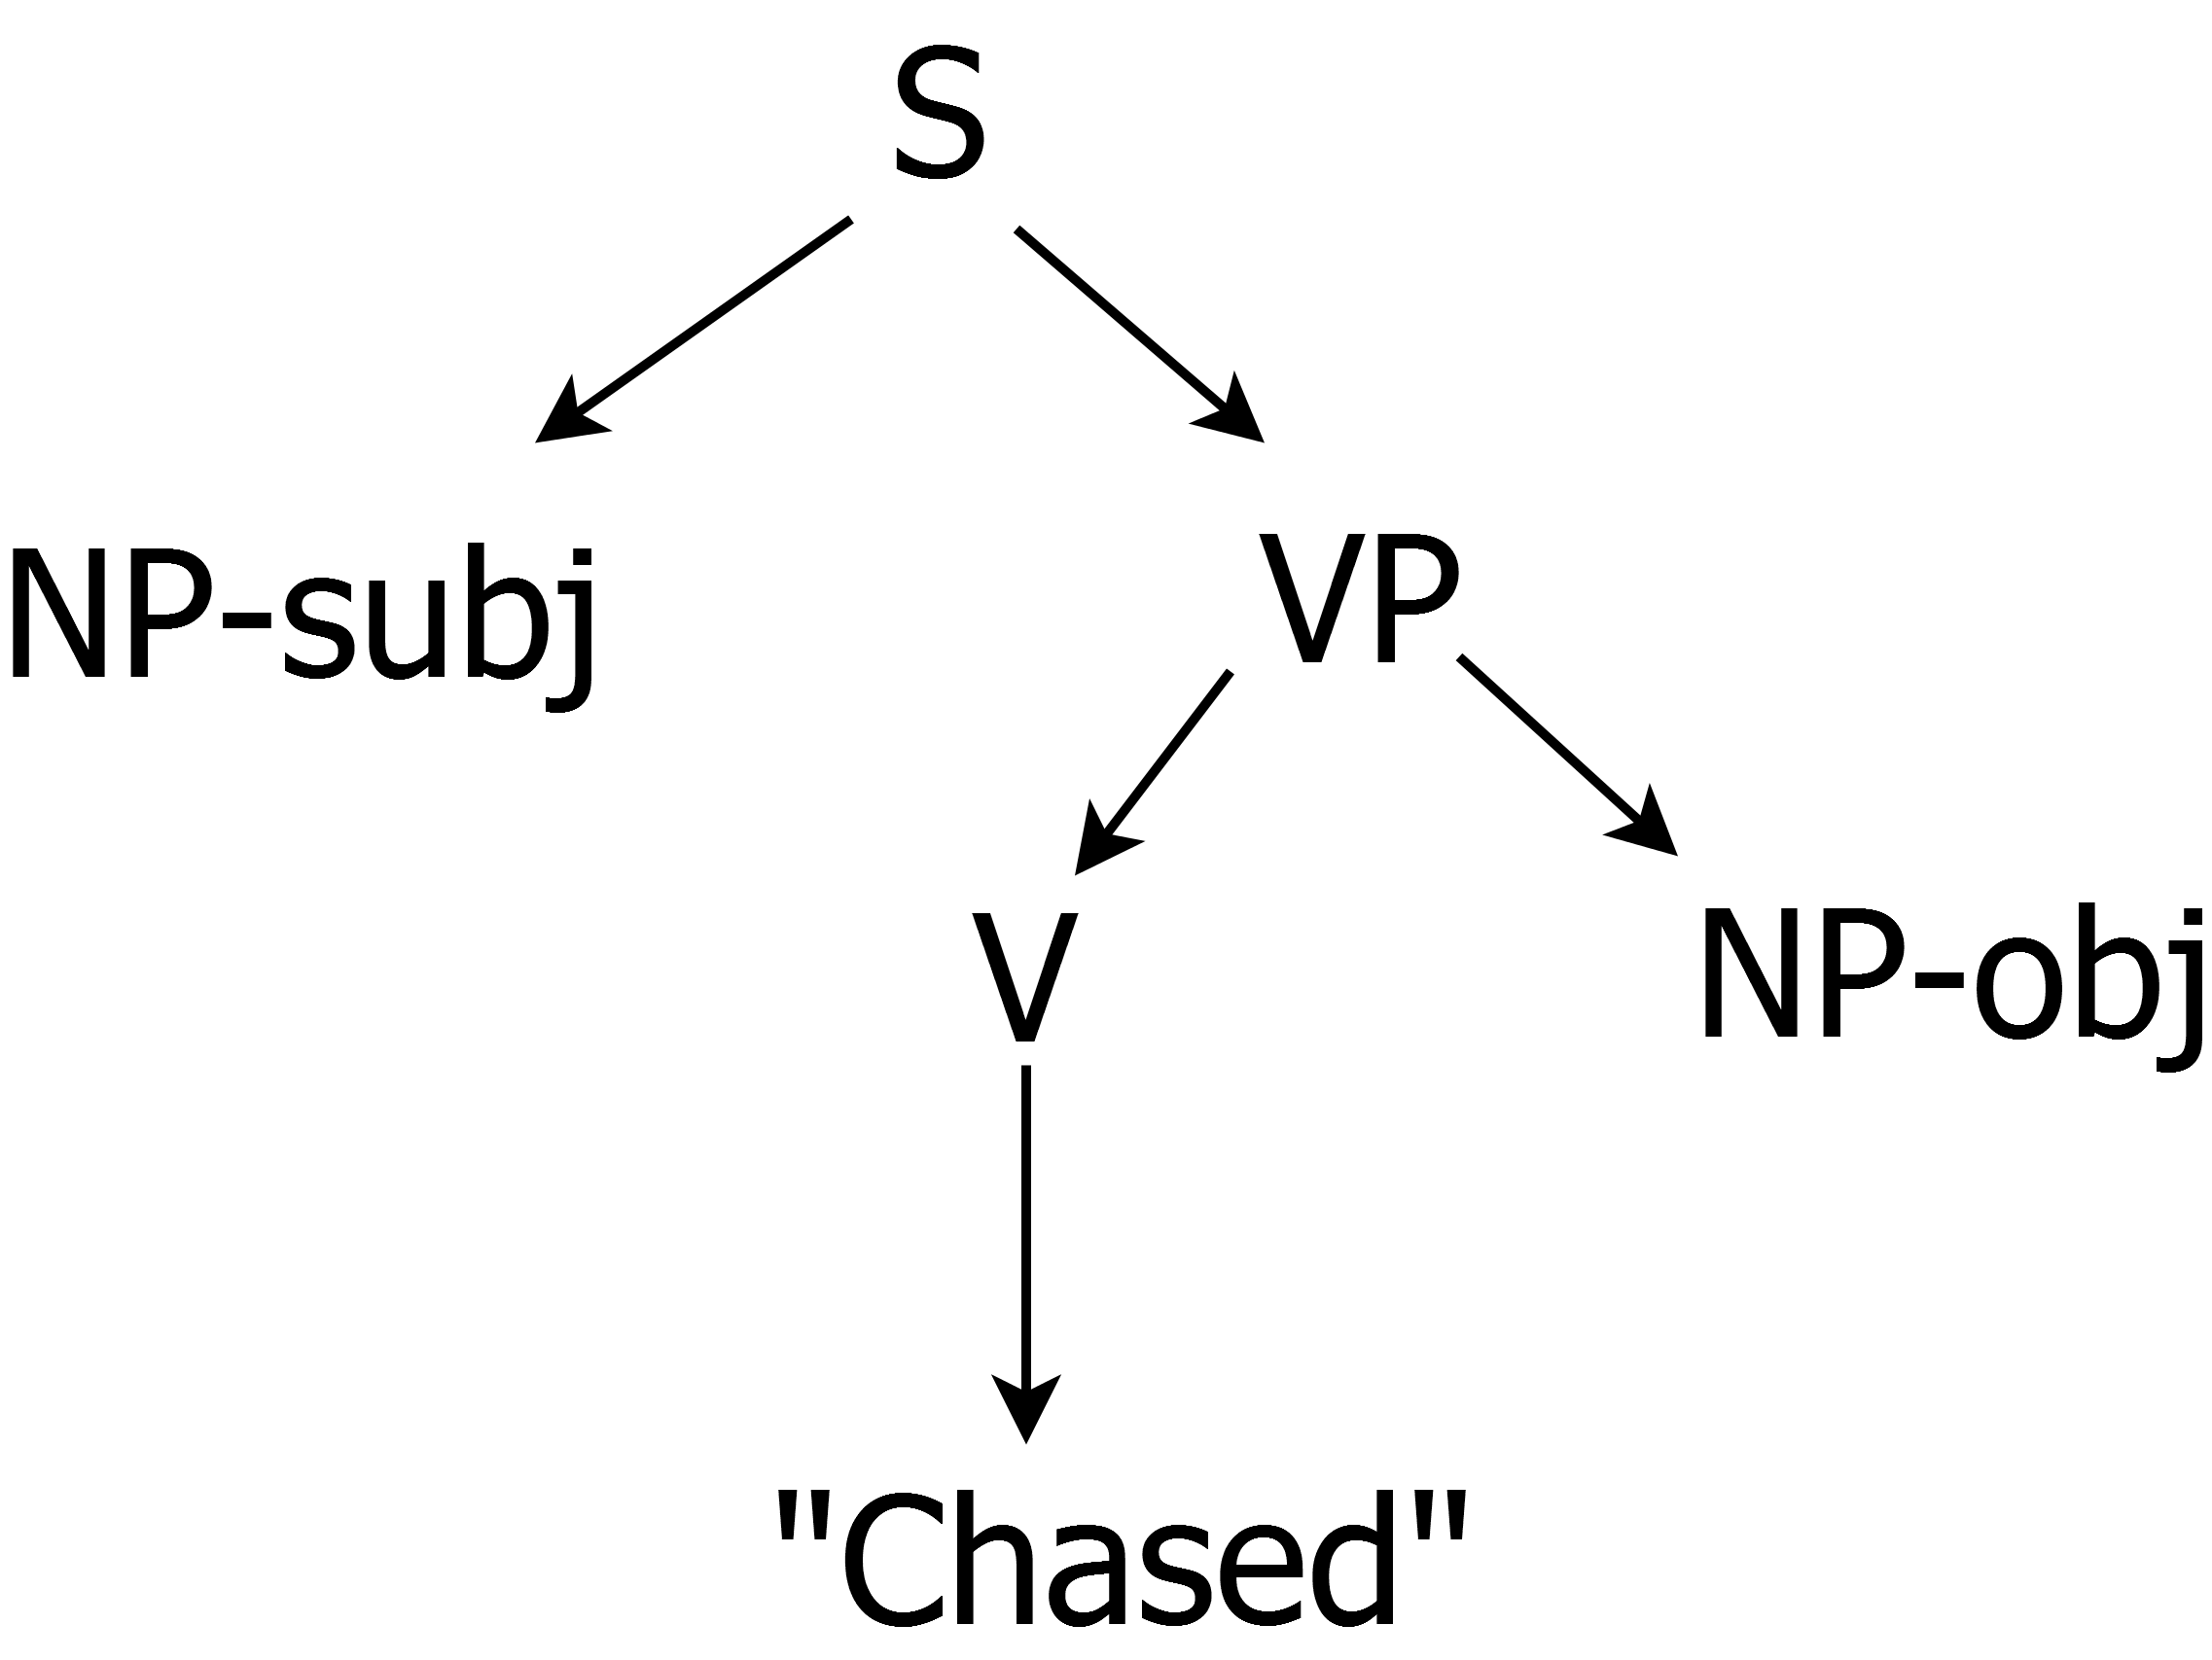
\includegraphics[width=.4\linewidth]{s-vpnp.png}
\caption{A tree in a STRUCT grammar, lexicalized and with entity annotations}
\label{s-to-npvp}
\end{figure}

\begin{figure}[t]
\centering
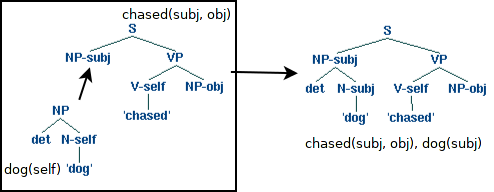
\includegraphics[width= 0.7 \linewidth]{sub-example.png}\label{examples-s}
\caption{An example tree substitution operation in STRUCT.}
\end{figure}

\begin{figure}[t]
\centering
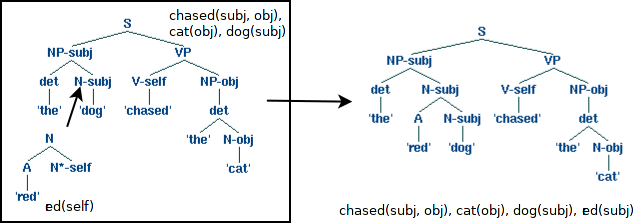
\includegraphics[width= 0.7 \linewidth]{adjoin-example.png}\label{examples-a}
\caption{An example tree adjoining operation in STRUCT.}
\end{figure}

In order to control the search space, we restrict the structure of the
MDP so that while substitutions are available, only those operations
are considered when determining the distribution over the next state,
without any adjoins.  This also allows us to generate a
complete and valid sentence quickly.  This allows STRUCT to operate as
an anytime algorithm, described further below.

From this point, we use a modified version of UCT
to plan in the MDP from the initial state specified above. 
Our choice of UCT is motivated by the high branching factor encountered in natural language generation when dealing with
large grammars as well as the belief that optimal sentences to accomplish a communicative goal are not required in most
discourse. In fact, generating optimal sentences may be more time-consuming than nearly-optimal plans which accomplish
the goal nearly as well.

\begin{algorithm}
\caption{The STRUCT$_a$ reward function.}\label{struct-a}
\begin{algorithmic}[1]
\REQUIRE State $s$, World $w$, Goal $g$
\ENSURE Numerical reward
\STATE $bestReward \gets$ -INF
\STATE $countValidPermutations \gets$ 0
\FOR {permutation $p$ of entities in the world}
	\STATE $currentReward \gets 0.0$
	\IF {all $prop$ in $s$, mutated by $p$, are in $w$}
		\STATE $currentReward \gets$ 10.0
		\STATE $countValidPermutations++$
	\ENDIF
	\IF {$g$ is satisfied by $s$ mutated by $p$}
		\STATE $currentReward += 50.0$
	\ENDIF
	\FOR {entity $e$ in $p$}
		\IF {$e$ is uniquely described by $s$, mutated by $p$}
			\STATE $currentReward += 1.0$
		\ENDIF
	\ENDFOR
	\IF {$currentReward > bestReward$}
		\STATE $bestReward \gets currentReward$
	\ENDIF
\ENDFOR
\IF {$countValidPermutations == 0$}
	\RETURN -INF
\ENDIF
\RETURN $bestReward / countValidPermutations$
\end{algorithmic}
\end{algorithm}

\begin{algorithm}
\caption{The STRUCT$_b$ reward function.}\label{struct-b}
\begin{algorithmic}[1]
\REQUIRE State $s$, World $w$, Goal $g$
\ENSURE Numerical reward
\STATE $maxReward \gets 0$
\FOR {entity $e$ in the world}
	\STATE $currentReward \gets 0$
	\STATE $possibleEntities \gets 0$
	\FOR {proposition $p$ in $s$}
		\FOR {entity $e_p$ in $p$}
		\IF {no proposition violates $p$ for $e$ = $e_p$}
			\STATE $possibleEntities++$
		\ENDIF
		\IF {no proposition violates $g$ for $e$ = $e_p$}
			\STATE $currentReward += 5$
		\ENDIF
		\ENDFOR
	\ENDFOR
	\IF {$possibleEntities == 0$}
		\STATE $currentReward \gets -INF$
	\ELSE
		\STATE $currentReward = currentReward / possibleEntities$
	\ENDIF
	\IF {$currentReward > maxReward$}
		\STATE $maxReward = currentReward$
	\ENDIF
\ENDFOR
\RETURN $maxReward$
\end{algorithmic}
\end{algorithm}

\subsection{Modifications to UCT}

We made three modifications to UCT in order to increase its usability
in the MDP we have defined.  This is motivated by the difference between
the initial purpose of UCT and the NLG application's needs.
UCT was originally used to search for sparse rewards
in a tree \cite{kocsis_bandit_2006}, where we are using it to search
for dense rewards in a DAG of potentially infinite depth.
Our reward functions may provide feedback after every action,
and a single simulation
may run for an arbitrary amount of time.
Consequently, we have implemented a depth limit
on our tree search.  We perform a number of actions in the
default policy stage of UCT equal to a parameter $d$.  We then
evaluate our reward function at the state we reach and push that
reward up to the root as usual.  This is motivated by the fact that the
first action taken will usually provide the greatest indication of the
quality of that branch.

This observation that we using a tree-search algorithm to search in a DAG
also brings up the question of reaching identical states
from two distinct parents.  STRUCT treats states which are otherwise
identical which are reached from different parents as different states.

Second, UCT is normally used in an environment where the transition
function is nondeterministic.  UCT is often used in an adversarial environment,
like chess or Go, and consequently searches for the best average case
from a given state.  In such cases,
selecting the absolute best may be risky if the opponent can respond
with something that can also lead to a very bad result. In our case,
however, there is no opponent, so we can freely choose the action
leading to best overall reward.

Third, UCT normally ends the tree policy phase by selecting an action
from the unexplored actions list randomly.  In the domain of NLG,
we know that there is additional information available to our system
regarding the value of an action, even before we take it. For instance,
when we are looking for an adjective to adjoin to 'sky', we know that 'blue' is
much more likely than 'red', even without evaluating our reward function.
STRUCT allows for a heuristic to order the nodes
it searches.

\subsection{Execution as an Anytime Algorithm}
 With the MDP definition above, we use UCT to find a solution sentence
 (Figure~\ref{struct-alg}). After every action is
 selected and applied, we check to see if we are in a state in which
 the algorithm could terminate (i.e. the sentence has no nonterminals
 yet to be expanded).  If so, we determine if this is the best
 possibly-terminal state we have seen so far.  If so, we store it, and
 continue the generation process. If we reach a state from which we
 cannot continue generating, we begin again from the start state of
 the MDP. Because of the structure restriction above (substitution
 before adjoin), STRUCT also generates a valid sentence quickly. These
 modifications enable STRUCT to perform as an anytime algorithm, which
 if interrupted will return the highest-value complete and valid
 sentence.

After this point, any time that there are no substitutions
available (all nonterminals have at least one child), we record the
current sentence and its associated reward.  Such a sentence is
guaranteed to be both grammatical and complete.  If generation is
interrupted, we return the highest-value complete and valid sentence.
In this way, our approach functions as an anytime algorithm.

See Algorithm \ref{uct-code} for the algorithm for a single generation.
We begin by looping until we have generated a complete sentence
(line 3).  We run $n$ simulations for each action selected (line 4),
during which we first apply any unexplored actions (line 7-9).  If
we still have available depth remaining after this (line 11), we will
apply actions as selected by PLTAG probability (line 12) until we
do not have any remaining allowable depth.  Afterwards, we will
calculate the reward for the state we've reached and propagate it
up the tree to the first action selected.  If the sentence is complete
(has no nonterminals without children), we will consider it as a candidate
for best anytime generation.  Then we will begin another
simulation.  After all the simulations are complete, we will select
the action which led to the best outcome (lines 22-24).  If we have
elected to emit the sentence, generation halts.

\begin{algorithm}
\caption{STRUCT simulation}\label{uct-code}
\begin{algorithmic}[1]
\REQUIRE Number of simulations $numTrials$, Depth of lookahead $maxDepth$
\ENSURE Generated sentence tree
\STATE $bestSentence \gets$ nil
\STATE $state \gets$ empty sentence tree
\WHILE{$state$ not terminal}
	\FOR{$numTrials$}
		\STATE $testState \gets state$
		\STATE $currentDepth \gets 0$
		\IF{$testState$ has unexplored actions}
			\STATE Apply one unexplored action chosen
                        with PLTAG probability at random to $testState$
			\STATE $currentDepth$++
		\ENDIF
		\WHILE{$currentDepth < maxDepth$}
			\STATE Apply action selected by tree
                        policy to $testState$
			\STATE $currentDepth$++
		\ENDWHILE
		\STATE calculate reward for $testState$
		\STATE associate reward with first action taken
		\IF {$testState$ is a complete sentence}
			\STATE consider $testState$ as a possibility for best anytime result.
		\ENDIF
	\ENDFOR
	\STATE $state \gets$ maximum reward $testState$
	\IF{$state$ score $> bestSentence$ score \AND $state$ has no nonterminal leaf nodes}
		\STATE $bestSentence \gets state$
	\ENDIF
\ENDWHILE
\RETURN $bestSentence$
\end{algorithmic}
\end{algorithm}

\begin{algorithm}
\caption{STRUCT Algorithm.} \label{struct-alg}
\begin{algorithmic}[1]
\REQUIRE Grammar $grammar$, World Description $w$, Goal $g$, Time Limit $t$
\ENSURE Generated sentence
\STATE $prunedGrammar \gets$ empty grammar
\STATE $necessaryEntities \gets$ empty list
\FOR {$entity$ in $w$}
	\IF {$e$ interacts with any entity in $g$, transitively}
		\STATE $necessaryEntities.append(e)$
	\ENDIF
\ENDFOR
\FOR {$tree$ in $grammar$}
	\IF {any proposition in $w$ applies $tree.meaning$ to any entity in $necessaryEntities$}
		\STATE $prunedGrammar.append(tree)$
	\ENDIF
\ENDFOR
\STATE $bestSentence \gets$ empty string
\STATE $bestScore \gets$ -INF
\WHILE {Time limit not expired}
	\STATE $score, sentence \gets STRUCT\_SIMULATION(prunedGrammar, w, g)$
	\IF {$score > bestScore$}
		\STATE $bestSentence \gets sentence$
		\STATE $bestScore \gets score$
	\ENDIF
\ENDWHILE
\end{algorithmic}
\end{algorithm}